
Synthetic data has become integral to language model training.
Instruction tuning, knowledge distillation, and data augmentation all routinely use model-generated text, and as synthetic corpora are recycled into training pipelines, the process often becomes recursive: each generation of models is fine-tuned on outputs from the previous one.
Recent work demonstrates that such recursive synthetic training triggers \textit{model collapse}, a progressive erosion of distributional tails and downstream capability~\citep{shumailov2024collapse, dohmatob2024tails, dohmatob2024demystified, alemohammad2024mad}.
The problem is especially pressing as web-scraped corpora increasingly contain model-generated content~\citep{dohmatob2025strong}, a trend that introduces implicit recursive loops even without deliberate data reuse.

While model collapse is now well-characterized through theoretical analysis~\citep{dohmatob2024tails, seddik2024synthetic} and empirical studies~\citep{shumailov2024collapse, alemohammad2024mad, gerstgrasser2024inevitable}, its effect on the geometric structure of learned representations~\citep{ethayarajh2019contextual, martin2021implicit} remains poorly understood.
Characterizing how the embedding space contracts during recursive training could yield computationally cheap collapse indicators from internal model states alone, without text generation or benchmark evaluation.

Current collapse detection depends on downstream metrics such as perplexity and benchmark accuracy, or on analysis of generated text through lexical diversity measures.
Both approaches require either costly inference or external evaluation infrastructure at every generation.
SIGMA~\citep{gu2026sigma} introduced spectral monitoring through embedding covariance analysis and showed that spectral indicators can track collapse, but validated only on OPT-125M over short generation horizons.
Four gaps remain open.
First, although spectral collapse has been linked to plasticity loss~\citep{he2025spectral} and rank collapse observed in attention layers~\citep{naderi2025mindgap}, no work has characterized spectral dynamics in recursive training beyond a few generations.
Second, the temporal relationship between spectral indicators and downstream degradation has not been examined.
Third, ecological early warning signals (EWS) theory warns that stabilization interventions can suppress the precursors they rely on~\citep{scheffer2009ews, scheffer2012anticipating}; whether this prevention--detectability tradeoff manifests in recursive model training---and how severely---has not been tested.
Fourth, while data mixing strategies are well-studied for pretraining~\citep{longpre2024pretrainer, xie2023doremi}, the relationship between real-data mixing ratios and spectral collapse has not been mapped: it is unknown how much real data suffices to prevent spectral contraction, or whether a sharp phase boundary exists.

We address these gaps by tracking spectral indicators of the embedding matrix across 10 recursive generations of Pythia-410M-deduped~\citep{biderman2023pythia}, with pilot validation on Pythia-1B-deduped and cross-architecture confirmation on GPT-2-medium~\citep{radford2019language}.
Our analysis reveals a reproducible three-phase pattern (Figure~\ref{fig:spectral_trajectory}): spectral decompression (Gen~0--2), where effective rank ($r_{\text{eff}}$)~\citep{roy2007effectiverank} and spectral log-volume (SLV) rise while downstream performance already declines; collapse onset (Gen~2--4), where spectral indicators reverse; and accelerating collapse (Gen~4--10), where contraction accelerates.
Among these indicators, SLV is the most effective collapse indicator: it requires only a forward pass on held-out data (no text generation), captures distributed volume changes across all spectral directions, and declines monotonically after its peak.
We further design a proportional controller as a testbed for reactive collapse prevention, uncovering a prevention--detectability tradeoff: the rate-based spectral signal degrades continuously as the real-data fraction increases and vanishes entirely above $r_{\text{crit}}$, leaving no regime where reactive control and effective prevention coexist.

Our contributions are:
\begin{itemize}
\item \textbf{C1:} The first multi-seed spectral-downstream characterization over 10 recursive generations, which reveals dynamics invisible in prior short-horizon studies and establishes a reproducible three-phase collapse pattern (decompression, onset, acceleration) (\S\ref{subsec:phase0}, Table~\ref{tab:phase0}).
\item \textbf{C2:} SLV as a computationally cheap collapse indicator with monotonic post-peak decline and a HellaSwag-spectral asymmetry: downstream degradation begins during the spectral decompression phase, so spectral expansion does not indicate model health (\S\ref{subsec:phase0}, \S\ref{subsec:alt_ews}).
\item \textbf{C3:} A prevention--detectability tradeoff: the spectral controller signal degrades continuously as the real-data fraction approaches $r_{\text{crit}}$ and vanishes entirely above it---a particularly strong form of the ecological intervention--warning tradeoff and, to our knowledge, the first quantification of this tradeoff in ML (\S\ref{subsec:controller}, \S\ref{subsec:phase1}).
\end{itemize}
Supporting these findings, we construct a spectral collapse trajectory map across multiple mixing ratios that localizes $r_{\text{crit}}$ empirically, with the bound robust to both the exponential moving average (EMA) smoothing parameter and random seed (\S\ref{subsec:phase_diagram}, \S\ref{subsec:phase1}, \S\ref{subsec:phase_diagram_exp}), and provide preliminary cross-architecture evidence that the three-phase trajectory generalizes to GPT-2-medium (\S\ref{subsec:cross_arch}).

\begin{figure}[t]
\centering
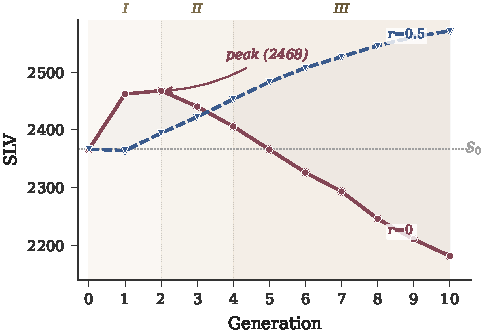
\includegraphics[width=\columnwidth]{figures/spectral_trajectory.pdf}
\caption{SLV across 10 recursive generations of Pythia-410M (solid: $r{=}0$, 3-seed mean; dashed: $r{=}0.5$, 2-seed mean) under pure-synthetic training and 50\% real-data mixing. Three phases are visible in the pure-synthetic trajectory: decompression (Gen~0--2, SLV peaks at 2468), onset (Gen~2--4), and acceleration (Gen~4--10, SLV falls 11.6\% from peak to 2181). Under 50\% mixing, SLV rises monotonically (except a negligible Gen~1 dip) to 2572 at Gen~10, 8.7\% above baseline and 104 points above the pure-collapse peak.}
\label{fig:spectral_trajectory}
\end{figure}
